\documentclass[letterpaper]{article} % DO NOT CHANGE THIS
\usepackage[submission]{aaai2027}  % DO NOT CHANGE THIS
\usepackage[hyphens]{url}  % DO NOT CHANGE THIS
\usepackage{graphicx} % DO NOT CHANGE THIS
\urlstyle{rm} % DO NOT CHANGE THIS
\def\UrlFont{\rm}  % DO NOT CHANGE THIS
\usepackage{natbib}  % DO NOT CHANGE THIS AND DO NOT ADD ANY OPTIONS TO IT
\usepackage{caption} % DO NOT CHANGE THIS AND DO NOT ADD ANY OPTIONS TO IT
\frenchspacing  % DO NOT CHANGE THIS
\usepackage{booktabs}

\pdfinfo{
/TemplateVersion (2027.1)
}

\setcounter{secnumdepth}{2}

\title{ContestBench: Do Medical LLMs Know When Physicians Disagree?}
\author{Anonymous Submission}
\affiliations{}

\begin{document}

\maketitle

\begin{abstract}
Every widely used benchmark for medical large language models assumes each
clinical question has a single correct answer. For a non-trivial fraction of
real medicine this is false: equally qualified physicians disagree, and that
disagreement is documented and clinically meaningful, not noise. A model that
answers a contested case with high confidence invites over-reliance exactly
where independent judgment is most needed, yet accuracy- and
calibration-based benchmarks cannot detect it, since they score confidence
against a gold label the case does not possess. We introduce
\textbf{ContestBench}, which replaces the binary gold label with the
empirical distribution of physician opinion. Using LIDC-IDRI, where four
radiologists independently rate each lung nodule, we derive a physician
\emph{agreement rate} $\pi \in [0.5,1]$ per case and score confidence by
\textbf{Physician Agreement Deviation (PAD)}, the L1 analogue of the Brier
proper scoring rule applied to a distributional target. We evaluate ten
model/reasoning configurations across three vendors on the full corpus
($n{=}1{,}413$) under one standardized elicitation. Confidence is linearly
uncorrelated with agreement (Pearson $r$ near zero everywhere) and only
weakly, inconsistently non-linearly dependent on it. A \textbf{case-blind
constant} (always $0.75$) achieves PAD $0.143$, and \textbf{all ten
configurations are significantly worse}. This is not because difficulty is
unpredictable: a predictor trained on the same rating-independent features
the models see attains PAD $\approx 0.127$, a \textbf{vignette-optimal}
target no model reaches. A post-hoc recalibrator mapping a model's own
confidence plus four cheap features onto $\pi$ closes almost the entire gap
for every configuration; an ablation shows confidence is statistically
redundant with those features for this purpose, though a small
independently-detectable signal survives. Extended reasoning does not help
(a mixed-sign null across five families), accuracy-based calibration
\emph{worsens} PAD for every configuration, in-context prompting closes the
gap only for the smallest model, and standard Expected Calibration Error is
uncorrelated with PAD and degenerate on exactly the cases the benchmark
targets. Finally, a reliance simulation shows PAD-minimizing recalibration
\emph{worsens} simulated over-reliance for models that were already
appropriately cautious, illustrating that optimizing an average calibration
metric is not the same as minimizing a safety-relevant downstream harm.
ContestBench and PAD give the field a measurement instrument for a failure
mode existing evaluation cannot see: LLM confidence decoupled from clinical
difficulty.
\end{abstract}

\section{Introduction}

\paragraph{A hidden assumption.} The benchmarks that govern medical LLM
development, MedQA \citep{jin2021medqa}, MedMCQA \citep{pal2022medmcqa}, and
their descendants \citep{medrbench2025,medthinkbench2025,li2024mediq}, share
an invisible premise: every clinical question has one correct answer against
which a model can be scored. This is false for a meaningful share of
clinical medicine. Inter-physician disagreement is extensively documented
and is not measurement error; it reflects genuine evidentiary uncertainty and
legitimate variation in expert judgment. Two equally experienced
radiologists can read the same chest CT and reach opposite conclusions
because the case is genuinely ambiguous, not because one is wrong.

\paragraph{Why it matters.} A model expressing high confidence on a
genuinely contested case fails in a specific, predictable way: it drives
over-reliance. A model that is uniformly confident regardless of difficulty
teaches users to either discount its confidence entirely or defer on
precisely the cases where independent judgment matters most -- the
automation-complacency failure mode documented in aviation and
decision-support research \citep{parasuraman1997humans}. No current
evaluation can detect this: accuracy benchmarks reward the confident answer
matching the gold label, and calibration metrics such as Expected
Calibration Error (ECE) require a binary correct/incorrect outcome that a
split physician panel does not provide. On exactly the cases needing
scrutiny, the standard tools are undefined or degenerate.

\paragraph{Our approach.} We measure confidence against the
\emph{distribution} of expert opinion rather than a single label, building
ContestBench on LIDC-IDRI \citep{armato2011lidc}, where four radiologists
independently rate each nodule's malignancy. From these ratings we compute a
per-case physician agreement rate $\pi = \max(f, 1-f) \in [0.5,1]$, $f$ being
the fraction rating the nodule malignant. A well-behaved model should be
confident when physicians agree ($\pi$ near $1$) and hedge when they split
($\pi$ near $0.5$). We quantify deviation from this ideal with
\textbf{Physician Agreement Deviation}, $\mathrm{PAD} = \mathrm{mean}|c -
\pi|$, the L1 form of the Brier proper scoring rule
\citep{brier1950verification,gneiting2007strictly} applied to a
distributional target. Every model is evaluated through one standardized
elicitation at full corpus scale ($n{=}1{,}413$), after confirming that
absolute PAD is elicitation-sensitive and cross-model comparison therefore
requires it held fixed.

\paragraph{What we find.} Model confidence does not track physician
agreement (correlation indistinguishable from zero; only half of
configurations show an MI excess surviving multiple-comparison correction).
A \textbf{case-blind constant} beats every one of ten configurations
significantly; a \textbf{vignette-optimal oracle} using only features
already in the models' prompts reaches PAD $\approx 0.127$, so the failure is
one of use, not access; \textbf{extended reasoning does not close the gap}
(mixed-sign, $|\Delta\mathrm{PAD}|\le0.033$ across five families, including a
DeepSeek-R1-lineage model); and \textbf{ECE cannot see any of this}. A
mechanism analysis rules out the benign story that confidence is noise:
models respond substantially to case features ($R^2$ up to $0.76$) but their
feature-to-confidence mappings contradict one another, and models do not
even agree on which cases are hard.

\paragraph{Contributions.} (1) \textbf{ContestBench}, scoring medical-LLM
confidence against a documented physician-agreement distribution rather than
a gold label, on a public, IRB-free corpus. (2) \textbf{PAD}, a
proper-scoring-rule-motivated metric for a distributional target, with a
demonstration that ECE is degenerate exactly where the benchmark is
informative and that accuracy-calibration does not imply
agreement-calibration. (3) A \textbf{full-scale, ten-configuration
evaluation} showing the decoupling is universal, that a cheap oracle beats
every model, and that reasoning and prompting do not close the gap. (4) A
\textbf{post-hoc recalibrator} that closes the oracle gap for every model,
paired with an over-reliance simulation showing this metric-optimal fix is
not automatically harm-optimal. (5) A \textbf{reproducible pipeline}
regenerable end to end from raw annotation files.

\section{Related Work}

\textbf{Single-label medical QA.} MedQA \citep{jin2021medqa} and MedMCQA
\citep{pal2022medmcqa}, their reasoning-focused successors
\citep{medrbench2025,medthinkbench2025}, and adaptive frameworks such as
MEDIQ \citep{li2024mediq} all score answers against a single correct choice.
ContestBench targets exactly the population -- genuinely contested cases --
for which this premise is false, asking not whether the model is right but
whether its confidence tracks how right an answer \emph{can be}.

\textbf{Learning from disagreement.} A parallel NLP line argues a single
ground truth discards annotator-disagreement information and proposes
training on soft labels instead \citep{davani2022dealing,uma2021learning}.
ContestBench reuses this insight for a different purpose: a
\emph{deployment-time evaluation instrument} with proper-scoring-rule
semantics, on annotators who are practicing physicians.

\textbf{Calibration in medicine and beyond.} ECE and its binning variants
\citep{guo2017calibration,naeini2015obtaining} and Platt scaling
\citep{platt1999probabilistic}, which we use as an accuracy-calibration
baseline, are all anchored to a single correct answer per case and are
undefined for a split panel. \citet{byun2026overconfidence} study
overconfidence and Platt-scaling in medical VQA; \citet{savage2025jamia} use
sample-consistency as a non-verbalized signal (reused here as a robustness
check, Section~\ref{sec:consistency}); \citet{testoni2026mindthegap} study
specialty-aware clinical-QA uncertainty. Our accuracy-calibration baseline
(Section~\ref{sec:acc-cal}) makes the distinction concrete: calibrating to
accuracy \emph{worsens} PAD for every configuration.

\textbf{Verbalized LLM confidence.} \citet{kadavath2022languagemodels} and
\citet{tian2023justask} study whether LLMs' stated confidence is
well-calibrated to correctness; \citet{xiong2024llmsexpress} benchmark
elicitation strategies, \citet{lin2022teaching} teach models to express
uncertainty in words, \citet{mielke2022reducing} reduce conversational
overconfidence via linguistic calibration, \citet{ovadia2019trust} evaluate
predictive uncertainty under distribution shift more broadly, and
\citet{jiang2021know,desai2020calibration} study calibration of pretrained
transformers and QA models. \citet{steyvers2025what} additionally show a
mismatch between what LLMs know and what users think they know. All target
correctness calibration or human perception of it; none address a
distributional target. \citet{singhal2023large} and clinical LLM evaluations
motivate our domain choice, and \citet{kompa2021second} motivate uncertainty
communication in medical ML as a deployment concern, which we operationalize
via the over-reliance simulation (Section~\ref{sec:reliance}), itself
building on an HCI literature showing AI explanations and confidence
signals do not reliably prevent overreliance in practice
\citep{bansal2021does,bucinca2021trust,passi2022overreliance}.

\textbf{Concurrent work.} \citet{medqade2026}, concurrent with this work,
finds physicians scale caution with difficulty while LLM judges evaluating
open-response answers do not -- complementary evidence from the
judge/evaluator side rather than the diagnostician side, in a different
domain and design (accuracy-anchored judge evaluation vs.\ our
proper-scoring-rule evaluation of the model as diagnostician).

\textbf{Prior work and scope.} PAD is the L1 analogue of the Brier score
\citep{brier1950verification}, itself a strictly proper scoring rule
\citep{gneiting2007strictly} in the forecast-evaluation tradition of
\citet{murphy1973vector} and \citet{degroot1983comparison}. That agreement
is partially predictable from case features is an unsurprising fact, not a
claim requiring novel methodology; our oracle and recalibrator
(Sections~\ref{sec:oracle},~\ref{sec:recal}) reuse it diagnostically, not
as a novel prediction method. Our over-reliance
simulation (Section~\ref{sec:reliance}) is anchored in \citet{lee2004trust}
and \citet{parasuraman1997humans}.

\section{The ContestBench Corpus}
\label{sec:corpus}

\subsection{Physician Agreement from LIDC-IDRI}
LIDC-IDRI \citep{armato2011lidc} is a public lung-CT corpus in which up to
four radiologists independently annotate each nodule, including a five-point
malignancy rating. No DICOM imagery is available; we parse the annotation
XML directly, extracting each reader-nodule's ROI polygon and its
malignancy, subtlety, spiculation, and margin ratings. Since a raw
\texttt{noduleID} is not globally unique across a scan's four reading
sessions, we match nodules by XML-native centroid proximity (in-plane
$<30$px, slice $<3$mm; frozen after confirming corpus size and tier
composition are stable within $\pm5\%$ across a $2\times$ range of
thresholds, Appendix~\ref{app:matcher}), retaining groups with $\geq3$
readers: $n{=}1{,}413$ nodules across $709$ scans.

We define $f$ as the fraction of readers rating malignancy $\geq3$ of $5$
(the LIDC-IDRI field convention), and agreement rate $\pi = \max(f,1-f) \in
[0.5,1]$ -- the fraction agreeing with the majority side. $\pi$, not $f$, is
the correct target: comparing confidence to $f$ directly is a category
error, since a correctly-confident model on a unanimous-benign case ($f{=}0$)
would register a spurious deviation. $\pi$ is discrete under 4-reader support
($\{.5,.75,1\}$; 3-reader nodules add the one new value $\{.667\}$), so we tier cases as
\textbf{high} ($n{=}546$), \textbf{contested} ($n{=}708$), and
\textbf{ambiguous} ($n{=}159$, structurally all exact 4-reader splits). An
exclusion audit (Appendix~\ref{app:matcher}) confirms drops are almost
entirely LIDC's inherent sub-3mm/uncharacterized marks. Appendix~\ref{app:threshold}
separately shows the baseline-beating result is robust to the $\geq3$
threshold choice, while the pooled correlation is not -- fully decomposed
there, not left as an open question.

\subsection{The Vignette Template and Its Collisions}
\label{sec:collision}
Each case is presented as a vignette reporting only mean subtlety,
spiculation, and margin (Section~\ref{sec:elicitation}). This coarseness has
a consequence we treat as core method, not a footnote: $1{,}413$ cases
collapse to $690$ distinct vignettes, and $\mathbf{54.8\%}$ (n=775) share an
identical vignette with a different-$\pi$ case (mean $\pi$-spread $0.30$),
which the model cannot distinguish by construction. We report the achievable
target as \textbf{vignette-optimal} rather than a model-agnostic ceiling
(Section~\ref{sec:oracle}), and confirm on the collision-free $45.2\%$
subset ($n{=}638$) that decoupling is not a collision artifact
(Section~\ref{sec:decoupling}). Appendix~\ref{app:data} gives worked example
vignettes, including a colliding pair.

\section{Method}

\subsection{Physician Agreement Deviation (PAD)}
\label{sec:pad}
For confidence $c \in [0,1]$ and agreement $\pi \in [0.5,1]$,
\[
\mathrm{PAD} = \frac{1}{n}\textstyle\sum_i |c_i - \pi_i|, \qquad
\mathrm{PAD}^+ = \frac{1}{n}\textstyle\sum_i (c_i - \pi_i),
\]
unsigned PAD as the headline statistic and signed PAD$^+$ as a directional
diagnostic by tier ($\mathrm{PAD}^2$ reported where noted). \textbf{Claim
(unverified proof).} We claim, without independent proof verification, that
PAD inherits a proper-scoring-rule guarantee: if $\pi$ is the calibrated
probability a random reader agrees with the majority, expected PAD is
minimized at $c=\pi$. We flag this, not the empirical results, as the
paper's one unconfirmed theoretical component.

\subsection{Elicitation and Provenance}
\label{sec:elicitation}
Every model receives the identical instruction: a Malignant/Benign answer
and a 0--100 confidence for a nodule described only by mean subtlety,
spiculation, and margin, as one JSON object. An earlier pilot mixed
pipe-delimited and JSON formats across models; we caught this before it
became load-bearing and standardized on one elicitation for the reported
panel. We evaluate ten configurations (Anthropic Haiku/Sonnet/Opus, Google
Gemini, DeepSeek, each standard/thinking); Anthropic and Gemini were
collected via logged APIs (model string, temperature where settable, prompt
hash per call), while DeepSeek is a documented manual-collection exception
(no usable API path). \textbf{Provenance correction, disclosed in full:} a
manual, uncontrolled-temperature pass was later re-collected via API;
Haiku's PAD rose substantially ($0.16{\to}0.35$--$0.36$) because the manual
interface had deceptively clustered confidence near the corpus-optimal
constant, while every other configuration was stable within hundredths of
PAD across both routes. We report only corrected, API-provenanced values;
this strengthens rather than weakens the central claim, since no substantive
conclusion depends on the one configuration that looked deceptively
well-calibrated under noisier collection. Gemini:standard reached $96\%$
coverage ($n{=}1{,}350$) after key-rotation retries -- a deliberate stop,
PAD stable at $0.178$--$0.180$ across every coverage level tried. All other
configurations reached $n\geq1{,}412$; manual and API artifacts and
per-call provenance logs are preserved.

\subsection{Vignette-Optimal Oracle}
\label{sec:oracle}
To measure recoverable signal, we fit a $5$-fold out-of-fold predictor of
$\pi$ at three feature levels: \textbf{geometry-only} (ROI extent, the only
feature with zero subjective input), \textbf{rating-independent} (subtlety,
spiculation, margin, extent -- independent of the malignancy rating
specifically, and exactly what the LLMs see), and \textbf{all-features}
(adds reader count and malignancy-extremity, which share source with $\pi$).
We check gradient-boosted (200 estimators, depth 3, lr $0.05$), ridge
($\alpha{=}1$), and linear estimators. This is the \textbf{vignette-optimal}
target -- the best performance achievable from the same coarse,
collision-prone text the models see (Section~\ref{sec:collision}), not a
model-agnostic bound.

\subsection{Post-Hoc Recalibrator}
\label{sec:recal}
We separately fit a per-configuration recalibrator mapping [model confidence
+ the four rating-independent features] onto $\pi$, same out-of-fold
protocol. Comparing oracle (features only) against recalibrator (features
$+$ confidence) on identical folds gives a bootstrap CI on confidence's
marginal contribution (Section~\ref{sec:recal-results}). Every stochastic
procedure here -- CV splits, bootstrap, permutation nulls -- uses a fixed
code-level seed; we report draw counts in prose and release the seeded code.

\section{Results}

\subsection{No Model Beats a Case-Blind Constant}
\label{sec:baseline}
The PAD-minimizing constant is $c^\ast{=}0.75$, $\mathrm{PAD}{=}0.143$.
Table~\ref{tab:panel} reports, per configuration, $n$, mean confidence,
$r(c,\pi)$, PAD, and the bootstrap-CI'd gap to $c^\ast$. Every gap's $95\%$
CI is strictly positive: \textbf{all ten configurations are significantly
worse than never looking at the case.} The best is Gemini:standard (PAD
$0.178$), indistinguishable from DeepSeek:thinking ($0.179$); an earlier,
uncorrected pass had reported Haiku:thinking ($0.157$) as best, superseded by
the provenance correction (Section~\ref{sec:elicitation}), which strengthens
rather than weakens this claim. Figure~\ref{fig:baseline} shows every PAD
against the constant and oracle.

\begin{table*}[t]
\centering
\setlength{\tabcolsep}{3.5pt}
\begin{tabular}{lrrrrl}
\toprule
config & $n$ & conf & $r(c,\pi)$ & PAD & gap vs.\ constant [95\% CI] \\
\midrule
haiku:standard    & 1412 & 0.53 & $+0.042$ & 0.357 & $+0.214$ [$+0.203$, $+0.227$] \\
haiku:thinking    & 1413 & 0.52 & $+0.083$ & 0.352 & $+0.210$ [$+0.197$, $+0.223$] \\
sonnet:standard   & 1413 & 0.67 & $-0.078$ & 0.193 & $+0.050$ [$+0.045$, $+0.055$] \\
sonnet:thinking   & 1413 & 0.71 & $-0.041$ & 0.182 & $+0.039$ [$+0.034$, $+0.043$] \\
opus:standard     & 1413 & 0.68 & $-0.076$ & 0.186 & $+0.043$ [$+0.038$, $+0.048$] \\
opus:thinking     & 1413 & 0.72 & $-0.069$ & 0.185 & $+0.042$ [$+0.037$, $+0.047$] \\
gemini:standard   & 1350 & 0.79 & $-0.078$ & 0.178 & $+0.035$ [$+0.029$, $+0.040$] \\
gemini:thinking   & 1413 & 0.66 & $+0.071$ & 0.209 & $+0.066$ [$+0.057$, $+0.075$] \\
deepseek:standard\textsuperscript{$\dagger$} & 1413 & 0.64 & $+0.258$ & 0.198 & $+0.055$ [$+0.049$, $+0.061$] \\
deepseek:thinking\textsuperscript{$\dagger$} & 1413 & 0.70 & $-0.065$ & 0.179 & $+0.036$ [$+0.032$, $+0.040$] \\
\bottomrule
\end{tabular}
\caption{Full-corpus panel results. $c^\ast=0.75$, $\mathrm{PAD}_{c^\ast}=0.143$. All ten gaps significant. $\dagger$: manual-collection route; others API-provenanced.}
\label{tab:panel}
\end{table*}

\begin{figure}[t]
\centering
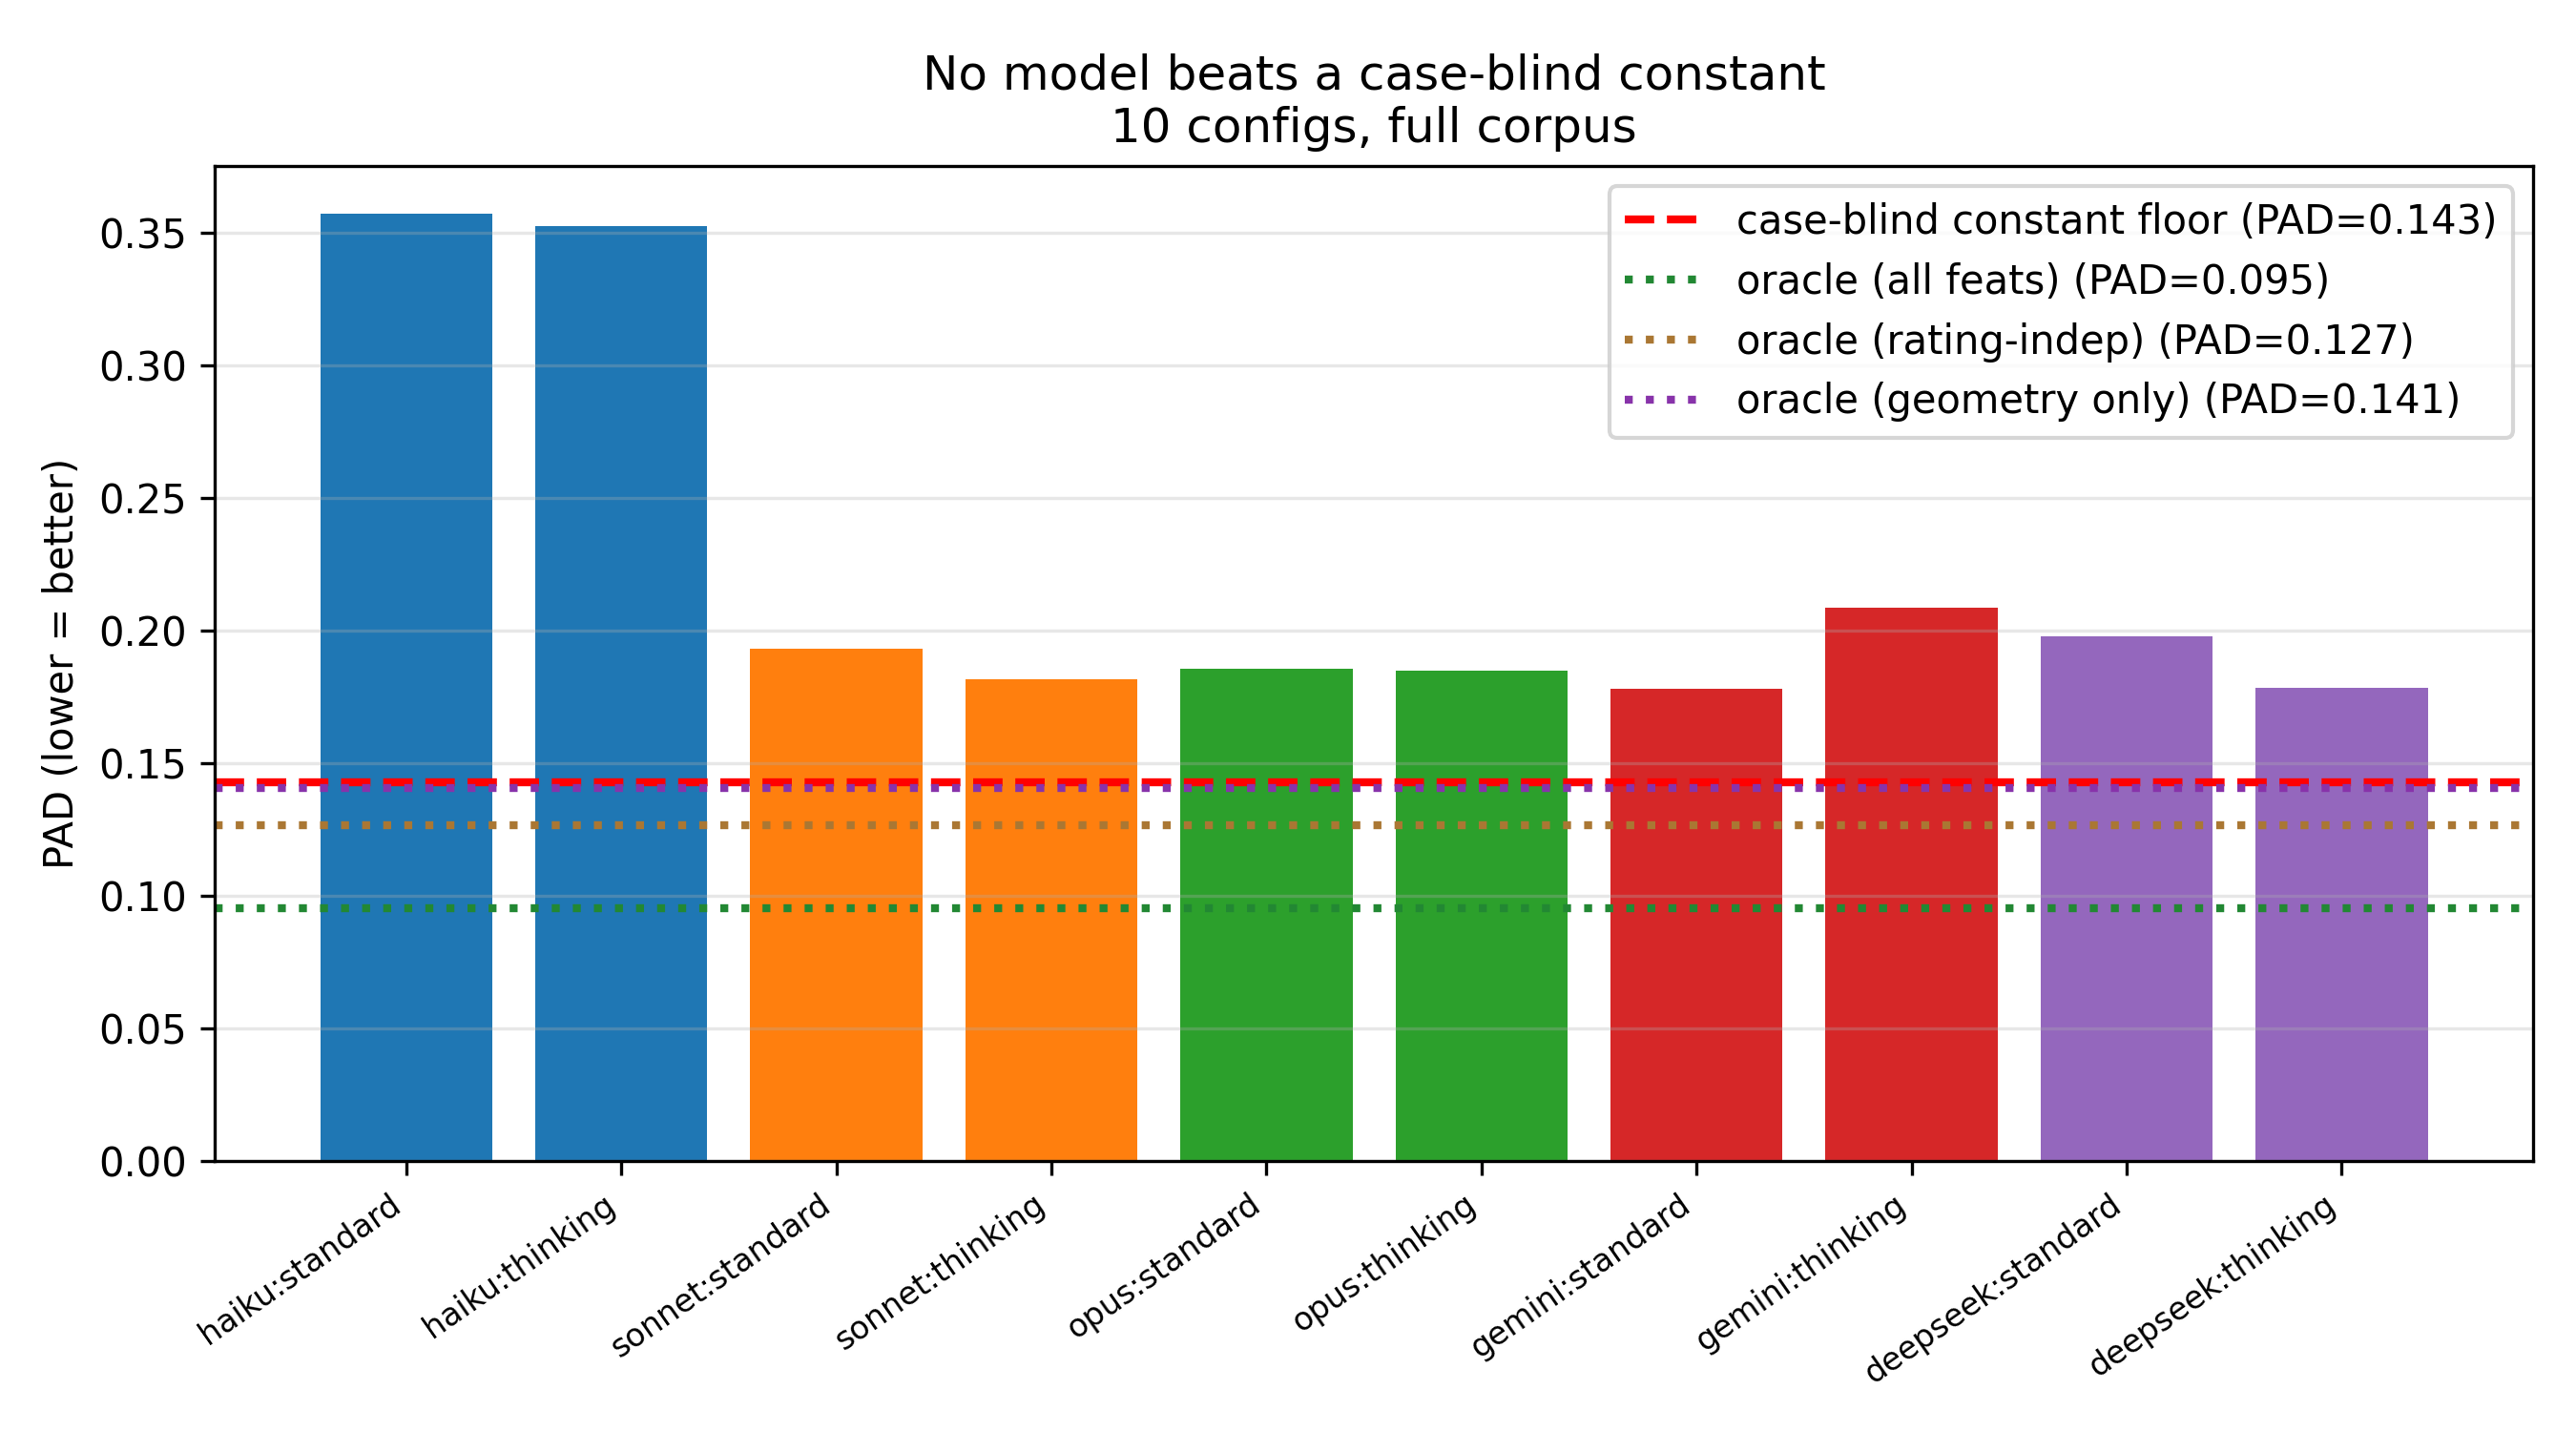
\includegraphics[width=0.95\columnwidth]{../results/figures/baseline_floor_all.png}
\caption{PAD per configuration against the case-blind constant floor (red) and the vignette-optimal oracle (dashed). No configuration reaches the constant.}
\label{fig:baseline}
\end{figure}

\subsection{Confidence Is Decoupled from Agreement}
\label{sec:decoupling}
Correlations are uniformly near zero ($-0.078$ to $+0.258$, Table~\ref{tab:panel}),
with confidence essentially flat while $\pi$ ranges over $[0.5,1]$. A
mutual-information test against a
$1{,}000$-permutation null ($k{=}3$ kNN, Table~\ref{tab:mi}) shows $8/10$
configurations exceed their null's $95$th percentile, but only $\mathbf{5/10}$
survive Bonferroni ($\alpha{=}0.005$); two (haiku:standard, sonnet:standard)
show no excess at $k{=}3$. This split is itself $k$-sensitive: at $k{=}5,10$,
three more configurations become significant, while sonnet:standard and
gemini:standard remain borderline at every $k$ ($p\in[0.004,0.02]$). The
defensible statement: confidence is linearly uncorrelated with agreement and
only weakly, inconsistently non-linearly dependent on it -- not flatly
independent, but not usably predictive. The oracle's own MI ($0.118$)
exceeds every model's. Restricting to the collision-free $45.2\%$ subset
($n{=}638$) reproduces the null (pooled $r{=}{+}0.07$), so this is not a
collision artifact.

The pooled near-zero correlation is also not uniform once cases are split by
sensitivity to the malignancy-positive threshold defining $\pi$: on the
$\approx61\%$ of cases whose tier flips between $\geq3$ and $\geq4$, the
correlation's \emph{sign} depends on which threshold is used (a composition
artifact of the redefinition, confirmed via the decomposition in
Appendix~\ref{app:threshold}, not a change in model output); on the
complementary $\approx39\%$ stable subset, four of five checked
configurations show a real, threshold-invariant \emph{positive} correlation
($+0.20$ to $+0.25$) that the pooled statistic averages away. We report the
pooled $\geq3$-threshold statistic as primary because $\geq3$ is the
field-standard convention, but flag this as a genuine refinement, not a
footnote.

\begin{table}[t]
\centering
\setlength{\tabcolsep}{3pt}
\small
\begin{tabular}{lrrrl}
\toprule
config & MI & excess & $p$ & Bonf.\ \\
\midrule
haiku:std    & 0.026 & $-0.008$ & 0.141 & no \\
haiku:think  & 0.025 & $+0.001$ & 0.045 & no \\
sonnet:std   & 0.013 & $-0.013$ & 0.189 & no \\
sonnet:think & 0.058 & $+0.030$ & 0.001 & \textbf{yes} \\
opus:std     & 0.057 & $+0.020$ & 0.001 & \textbf{yes} \\
opus:think   & 0.038 & $+0.009$ & 0.020 & no \\
gemini:std   & 0.042 & $+0.015$ & 0.007 & no \\
gemini:think & 0.123 & $+0.089$ & 0.001 & \textbf{yes} \\
deepseek:std & 0.095 & $+0.054$ & 0.001 & \textbf{yes} \\
deepseek:think & 0.091 & $+0.056$ & 0.001 & \textbf{yes} \\
\midrule
oracle & 0.118 & $+0.092$ & 0.001 & -- \\
\bottomrule
\end{tabular}
\caption{MI(confidence,$\pi$), $k{=}3$, vs.\ permutation null; excess = MI $-$ null 95th pct. Bonferroni $\alpha{=}0.005$, $5/10$ survive.}
\label{tab:mi}
\end{table}

\subsection{The Vignette-Optimal Oracle Beats Every Model}
\label{sec:oracle-results}
Table~\ref{tab:oracle} reports oracle PAD across feature levels and
estimators. Rating-independent (features already shown to every LLM)
attains $\mathrm{PAD}\approx0.127$--$0.133$ robustly, beating every model
(best $0.178$). The all-features headline ($0.095$) is GBT-specific (ridge/
linear: $0.131$); geometry alone ($0.139$--$0.141$) is indistinguishable
from the constant, so the signal lives in subjective Likert calls, not raw
size. A leave-one-out bucket-mean baseline (no fitting) gives $0.140$
(indistinguishable from the constant); in-sample is $0.067$ but leaky.
\textbf{Conclusion:} the vignette affords only $0.010$--$0.016$ PAD of
usable margin over ignoring the case, depending on estimator, real and
achievable from the same prompt the models see -- and no model captures any
of it.

\begin{table}[t]
\centering
\small
\begin{tabular}{lrrr}
\toprule
oracle variant & gbt & ridge & linear \\
\midrule
geometry-only            & 0.141 & 0.139 & 0.139 \\
rating-independent       & 0.127 & 0.133 & 0.133 \\
all-features$^\dagger$   & 0.095 & 0.131 & 0.131 \\
\midrule
bucket-mean (LOO) & \multicolumn{3}{c}{0.140} \\
case-blind constant      & \multicolumn{3}{c}{0.143} \\
best evaluated model     & \multicolumn{3}{c}{0.178} \\
\bottomrule
\end{tabular}
\caption{Oracle PAD, 5-fold out-of-fold. $\dagger$: shares source with $\pi$; $0.095$ is GBT-specific.}
\label{tab:oracle}
\end{table}

\subsection{Mechanism: What Drives Confidence Instead}
Confidence is not noise: OLS on the locked feature set attains $R^2$ from
$0.054$ (haiku:standard) to $0.758$ (deepseek:standard). Haiku's low $R^2$ is
consistent with its provenance-corrected confidence being noisier, a
data-quality artifact of that configuration, not evidence the analysis is
compromised elsewhere. Feature-to-confidence mappings \emph{contradict}
across models (e.g., the spiculation coefficient is strongly positive in one
configuration, strongly negative in another), and pairwise cross-model
confidence correlation spans $-0.30$ to $+0.84$ (mean $+0.27$): models do not
agree on which cases are hard, ruling out a shared latent difficulty signal
and pointing instead to idiosyncratic, model-specific heuristics.

\subsection{Post-Hoc Recalibration and the Confidence Ablation}
\label{sec:recal-results}
Table~\ref{tab:recal} shows the recalibrator closes essentially the entire
oracle gap for every configuration (raw PAD $0.178$--$0.357 \to
0.125$--$0.127$, matching the oracle's $0.127$), and gives the ablation:
comparing features-only against features$+$confidence on identical folds,
mean gap $+0.0007$ PAD, with $8/10$ configurations' bootstrap CI bracketing
zero. Two (haiku:standard, sonnet:standard) exclude zero, but by
$\approx0.0016$ PAD, an order of magnitude below any other effect in this
paper. Held-out permutation importance of confidence is small but non-zero
for most configurations (mean $0.023$, range $0.004$--$0.064$).
\textbf{Non-contradictory claim:} confidence is statistically redundant with
four cheap features for this purpose -- its marginal PAD contribution is
indistinguishable from zero for most configurations, negligible even where
technically significant -- while still carrying a small, real,
importance-detectable signal that is almost entirely redundant with those
features. The recalibrator succeeds by routing \emph{around} confidence, not
extracting from it.

\begin{table*}[t]
\centering
\small
\setlength{\tabcolsep}{4pt}
\begin{tabular}{lrrrl}
\toprule
config & before & after & closed & ablation gap [95\% CI] \\
\midrule
haiku:std    & 0.357 & 0.127 & 100\% & $+0.0016$ [$+0.0002$, $+0.0030$]$^\ast$ \\
haiku:think  & 0.352 & 0.126 & 100\% & $+0.0007$ [$-0.0008$, $+0.0022$] \\
sonnet:std   & 0.193 & 0.125 & 102\% & $+0.0017$ [$+0.0002$, $+0.0031$]$^\ast$ \\
sonnet:think & 0.182 & 0.127 & 100\% & $+0.0004$ [$-0.0007$, $+0.0017$] \\
opus:std     & 0.186 & 0.126 & 101\% & $+0.0003$ [$-0.0009$, $+0.0016$] \\
opus:think   & 0.185 & 0.126 & 100\% & $+0.0002$ [$-0.0011$, $+0.0015$] \\
gemini:std   & 0.178 & 0.127 & 100\% & $-0.0005$ [$-0.0019$, $+0.0010$] \\
gemini:think & 0.209 & 0.127 & 100\% & $+0.0005$ [$-0.0010$, $+0.0019$] \\
deepseek:std & 0.198 & 0.126 & 101\% & $+0.0000$ [$-0.0009$, $+0.0010$] \\
deepseek:think & 0.179 & 0.126 & 101\% & $+0.0006$ [$-0.0004$, $+0.0015$] \\
\bottomrule
\end{tabular}
\caption{Recalibrator PAD before/after and \% of the oracle gap (0.127) closed, with the paired ablation gap = PAD(features only) $-$ PAD(features+confidence). $^\ast$: CI excludes zero.}
\label{tab:recal}
\end{table*}

\subsection{Prompting Does Not Fix It}
\label{sec:intervention}
We test whether in-context exemplars shift confidence toward $\pi$ (three
designs: A, an explicit rule; B, a qualitative hedge; C, worked examples;
crossed with Haiku/Sonnet/Opus, on a shared, leak-free $300$-case held-out
set). Table~\ref{tab:intervention}: \textbf{Haiku improves under all three}
(PAD $0.356\to0.141$--$0.168$), reaching statistical parity with the
constant under B/C -- the one case where an intervention reaches (not
exceeds) the naive baseline. \textbf{Sonnet and Opus are largely inert or
worse}: their best design (B) narrows the gap (PAD $0.158$) but remains
significantly worse than the constant; Opus is actively hurt by C ($0.184\to
0.204$). No combination significantly beats the constant; prompting is not a
fix, the recalibrator is.

\begin{table}[t]
\centering
\small
\begin{tabular}{llrrl}
\toprule
model & design & before & after & vs.\ constant \\
\midrule
haiku  & A & 0.356 & 0.168 & worse$^\ast$ \\
haiku  & B & 0.356 & 0.147 & tied \\
haiku  & C & 0.355 & 0.141 & tied \\
sonnet & A & 0.188 & 0.186 & worse$^\ast$ \\
sonnet & B & 0.188 & 0.158 & worse$^\ast$ \\
sonnet & C & 0.188 & 0.189 & worse$^\ast$ \\
opus   & A & 0.184 & 0.189 & worse$^\ast$ \\
opus   & B & 0.184 & 0.158 & worse$^\ast$ \\
opus   & C & 0.184 & 0.204 & worse$^\ast$ (hurts) \\
\bottomrule
\end{tabular}
\caption{Prompting-intervention table, $n{=}300$ held-out, constant PAD$=0.143$. $^\ast$: gap CI excludes zero; ``tied'' brackets zero.}
\label{tab:intervention}
\end{table}

\subsection{Reasoning Effect: A Null Result}
Toggling thinking changes PAD by a small amount everywhere; unlike every
other comparison here, we give paired bootstrap $95\%$ CIs rather than
points alone: haiku $-0.005$ [$-0.014,+0.004$] (ns), sonnet $-0.011$
[$-0.015,-0.008$] (sig.), opus $-0.001$ [$-0.004,+0.003$] (ns), gemini
$+0.033$ [$+0.024,+0.043$] (sig.), deepseek $-0.019$ [$-0.025,-0.013$]
(sig.). Three of five show a detectable effect, but direction is
inconsistent and every estimate is far smaller than any other effect in this
paper. Reasoning neither fixes nor meaningfully worsens the decoupling,
across five families including a DeepSeek-R1-lineage model.

\subsection{Capability Trend (Suggestive)}
\label{sec:capability}
Within the Anthropic family, signed PAD on the ambiguous tier trends upward
with capability rank -- more-capable models are more confidently wrong on
exactly the cases physicians split on. We report this as suggestive only
(three rungs, non-monotonic, Opus-driven); full numbers in
Appendix~\ref{app:capability}.

\subsection{ECE Cannot See the Problem}
ECE and PAD are near-uncorrelated: gpt-oss-20b -- a supplementary,
differently-elicited model (single-call JSON, not the ten-panel's
pipe-batch format, so not directly comparable to Table~\ref{tab:panel}) --
has excellent accuracy-calibration ($\mathrm{ECE}{=}0.050$) alongside poor
agreement-calibration ($\mathrm{PAD}{=}0.170$, worse than the constant). ECE
is additionally degenerate on the ambiguous tier, requiring a binary label a
$50/50$ split does not provide: assigning that label at random across
$2{,}000$ draws swings ECE across a $0.15$-wide $95\%$ band, while PAD needs
no label and is a single stable value.

\subsection{Accuracy-Calibration Is Not Agreement-Calibration}
\label{sec:acc-cal}
Platt-scaling each configuration's confidence to its own accuracy (5-fold
CV, no leakage) and re-measuring PAD against $\pi$ \emph{worsens} PAD for
\textbf{every configuration}: pooled mean PAD rises $0.222\to0.368$.
Calibrating to a binary correctness label, the object it is designed for,
provably cannot calibrate confidence to physician agreement.

\subsection{Robustness Check: Non-Verbalized Confidence}
\label{sec:consistency}
On a reduced spot-check (two models, $n{=}56$--$85$), a genuinely
non-verbalized signal in the spirit of self-consistency and
consistency-based hallucination detection
\citep{wang2023selfconsistency,manakul2023selfcheckgpt} -- sample-consistency
across repeated draws, an approach to uncertainty estimation distinct from a
model's own stated confidence \citep{malinin2021uncertainty} -- reproduces
the null, with answer-saturation itself corroborating decoupling in raw
answer-space. Full numbers and caveats: Appendix~\ref{app:consistency}.

\subsection{Over-Reliance: A Second-Order Metric-Design Point}
\label{sec:reliance}
Following \citet{lee2004trust}, a clinician relies on the model's answer
with probability $\sigma(\beta(c-\theta))$; warranted reliance is $\pi$;
over-reliance is $\mathrm{mean}\max(0,P(\mathrm{rely})-\pi)$, averaged over
$\theta\in\{.5,.6,.7,.8\}$, $\beta\in\{5,10,20\}$, pooled across all ten
configurations. Decoupled confidence gives over-reliance $0.048$; ideal
($c{=}\pi$) gives $0.028$ ($41\%$ lower). The recalibrator, despite closing
the PAD gap for every configuration, lands at $\mathbf{0.070}$ --
\emph{worse} than raw pooled ($45\%$ higher) -- because it regresses every
configuration toward the oracle's residual mean, helping only the worst raw
configuration (gemini:standard, $0.087{\to}0.070$) and hurting the other
nine, most dramatically the cautious deepseek:standard
($0.025{\to}0.070$). This ranking holds at every one of the twelve
$(\theta,\beta)$ cells individually. \textbf{We read this as a genuine
second-order contribution:} PAD-minimization is not
over-reliance-minimization -- optimizing an average calibration metric can
move a safety-relevant quantity the wrong way for models that were already
appropriately cautious, a distinction invisible to any purely average-based
metric alone.

\begin{table}[t]
\centering
\small
\begin{tabular}{lrr}
\toprule
config & raw & recalibrated \\
\midrule
haiku:std    & 0.044 & 0.070 \\
haiku:think  & 0.039 & 0.070 \\
sonnet:std   & 0.039 & 0.069 \\
sonnet:think & 0.052 & 0.070 \\
opus:std     & 0.045 & 0.070 \\
opus:think   & 0.060 & 0.069 \\
gemini:std   & 0.087 & 0.070 \\
gemini:think & 0.044 & 0.070 \\
deepseek:std & 0.025 & 0.070 \\
deepseek:think & 0.050 & 0.070 \\
\midrule
pooled            & 0.048 & 0.070 \\
ideal ($c=\pi$)   & \multicolumn{2}{c}{0.028} \\
\bottomrule
\end{tabular}
\caption{Simulated over-reliance, raw vs.\ recalibrated. Helps only 1/10 configurations.}
\label{tab:reliance}
\end{table}

\section{Discussion}
The picture is confidence tracking something other than clinical difficulty:
models respond to features with real power ($R^2$ up to $0.76$) but in
contradictory, model-specific ways that align poorly with physician
disagreement, suggesting an architectural or training-level fix, not an
elicitation-level one -- neither reasoning nor prompting closes the gap,
while a trivial recalibrator does, cheaply, by ignoring confidence almost
entirely: useful, but an unflattering diagnosis. Section~\ref{sec:reliance}
complicates ``ship the recalibrator'': a metric-optimal fix is not
automatically harm-optimal. The capability trend
(Section~\ref{sec:capability}) raises, without confirming, a further
concern: if more-capable models are more confidently wrong on the hardest
cases, scaling capability without fixing the decoupling could worsen
over-reliance.

\section{Limitations and Broader Impact}
\textbf{Construct validity.} Tiers follow directly from LIDC-IDRI ratings
without independent clinical review against radiologists' own sense of
difficulty -- the largest open risk here, stated as unresolved.
\textbf{Single domain.} LIDC-IDRI is our only source; we checked five
BI-RADS-style candidates (VinDr-Mammo, CMMD, a Zenodo contrast-enhanced set,
an inaccessible 101-radiologist study, CBIS-DDSM), rejecting all as
consensus-only or inaccessible per-reader. \textbf{Text, not images;
discrete $\pi$; DeepSeek manual-only.} No DICOM was available, so models
reason over extracted features, not raw CT; $\pi$'s discreteness is
mitigated by the tier redefinition and collision-free-subset check, though a
continuous source would sharpen every result; DeepSeek is flagged
throughout as manual-collection only.
\textbf{Theorem~1 is unverified} (Section~\ref{sec:pad}).
\textbf{The pooled correlation is threshold-sensitive by a confirmed
mechanism} (Appendix~\ref{app:threshold}): concentrated in the
$\approx61\%$ tier-flipping subset, with a genuine positive signal on the
stable $\approx39\%$ averaged away in the pooled statistic -- a refinement,
not an unresolved risk. \textbf{Vignette richness.} Only
subtlety/spiculation/margin are used; unused LIDC-IDRI fields (calcification,
sphericity, lobulation, texture) could shrink the collision rate and raise
the oracle target, but we did not re-run the full panel against them.
\textbf{Availability.} Pipeline code and the derived corpus will be released
publicly upon publication under a research-use license.

\appendix
\section{Data Appendix: Example Vignettes and Corpus Statistics}
\label{app:data}
$n{=}1{,}413$ nodules, $709$ scans ($907$ four-reader, $506$ three-reader).
Tiers: high $546$, contested $708$, ambiguous $159$. Feature ranges
(1--5 LIDC scale; extent in px): subtlety $[1,5]$ (mean $3.92$), spiculation
$[1,5]$ (mean $1.61$), margin $[1,5]$ (mean $3.99$), extent $[8.0,88.6]$
(mean $21.9$). Only $690/1{,}413$ vignettes are unique
(Section~\ref{sec:collision}). One representative case, exact prompt
format: \textbf{High} ($\pi{=}1.0$, unanimous, 4 readers): ``subtlety 4.50 |
spiculation 2.50 | margin 4.00.'' A genuine collision from the corpus:
cases 581:4 and 581:5 share the identical presented vignette ``subtlety
2.25 | spiculation 1.00 | margin 2.75'' (both 4 readers), yet 581:4 is
ambiguous ($\pi{=}0.5$) and 581:5 is contested ($\pi{=}0.75$) -- the model
sees one prompt for two different agreement targets, illustrating
Section~\ref{sec:collision}'s caveat with a real corpus pair.

\section{Corpus and Matcher Robustness}
\label{app:matcher}
Matcher stability across tight ($20$px/$2$mm), base ($30$px/$3$mm, frozen
default), and loose ($40$px/$4$mm) thresholds: total size swings $\pm3\%$
($1{,}375$--$1{,}418$); the thinnest tier (ambiguous) moves $152$--$161$
cases ($\pm5\%$) while remaining essentially the same nodule set (Jaccard
$\geq0.94$). Tier assignment is not a hidden researcher degree of freedom.
An exclusion audit shows dropped annotations are $>99.9\%$ LIDC's inherent
sub-3mm/uncharacterized marks, not a pipeline artifact.

\section{Malignancy-Threshold Sensitivity}
\label{app:threshold}
$\pi$ depends on a threshold ($\geq3$ throughout, the LIDC field convention).
Recomputing at the stricter $\geq4$ threshold (same $1{,}413$ cases, pure
relabeling): $\pi$ changes for $61.5\%$ of cases, the high tier grows
$546{\to}728$, and $c^\ast$ moves to $1.0$ (PAD $0.162$). The baseline result
is robust (10/10 still worse than the $\geq4$ constant); the pooled
correlation is not (e.g., sonnet:standard $-0.078{\to}+0.271$). Three cheap
diagnostics, no re-query, resolve why: \textbf{(1)} confidence/answer
columns are identical across both analyses, so any shift is $\pi$-side;
\textbf{(2)} splitting cases into threshold-stable ($n{\approx}544$, $\pi$
literally identical under both thresholds) vs.\ threshold-sensitive
($n{\approx}869$) shows the shift is entirely in the sensitive subset,
where correlation sign flips with the threshold on identical confidences
(Table~\ref{tab:threshold-decomp}), while the stable subset shows a real,
invariant positive correlation ($+0.20$--$0.25$ for four of five
configurations) the pooled statistic averages away; \textbf{(3)} MI
corroborates this -- opus/gemini/deepseek:standard keep significant MI at
both thresholds, while sonnet:standard shows none at either despite its
large Pearson swing, confirming that swing is a linear-correlation
artifact. \textbf{Resolution:} a confirmed, characterized composition
effect, not an open mystery; we report the $\geq3$ field-standard statistic
as primary and treat this as a genuine qualification of the decoupling
claim.

\begin{table}[t]
\centering
\small
\begin{tabular}{lrrr}
\toprule
config & $r$ stable & $r_{\geq3}$ sens.\ & $r_{\geq4}$ sens.\ \\
\midrule
sonnet:std   & $+0.247$ & $-0.294$ & $+0.286$ \\
opus:std     & $+0.237$ & $-0.292$ & $+0.294$ \\
gemini:std   & $+0.201$ & $-0.291$ & $+0.201$ \\
haiku:std    & $+0.082$ & $+0.008$ & $-0.060$ \\
deepseek:std & $+0.238$ & $+0.214$ & $-0.240$ \\
\bottomrule
\end{tabular}
\caption{Correlation decomposition: threshold-stable (single column, identical under both thresholds) vs.\ threshold-sensitive under each threshold.}
\label{tab:threshold-decomp}
\end{table}

\section{Capability Trend: Full Results}
\label{app:capability}
Standard slope $+0.067$ ($95\%$ CI $[+0.044,+0.091]$); thinking $+0.095$
($[+0.072,+0.119]$); $n{=}159$ shared ambiguous cases, cluster-bootstrapped.
Three rungs only, non-monotonic (Sonnet below Haiku on some measures),
Opus-driven; strengthening this would need a multi-vendor capability ladder
at paid-API scale we did not have -- an acknowledged scope limit, not an
open action item.

\section{Non-Verbalized Confidence: Full Results}
\label{app:consistency}
Gemini, $10$ samples at temperature $0.8$ on $73$ cases, confidence =
fraction agreeing with the modal answer: reproduces the null ($r{=}-0.111$,
$95\%$ CI $[-0.305,+0.145]$, $p{=}0.35$), saturated $0.947$--$1.00$ across
tiers -- the model gives the same answer nearly every time even on a
$50/50$ case, corroborating decoupling in raw answer-space. A gpt-oss
spot-check (e5-embedded rationale cosine similarity) gives a similarly
flat, non-significant result. Caveats: small, single-model-per-variant
samples, partial completion ($n{=}56$--$85$), free-tier constraints;
directionally corroborating, not paper-grade precision.

\section*{Ethical Statement}
ContestBench is a measurement instrument, not a diagnostic tool; no
evaluated model is validated for clinical use. Our purpose is to surface a
failure mode -- confidence decoupled from clinical difficulty -- that could
encourage inappropriate trust where judgment matters most. Two-sided risk:
this could be misread as license to distrust LLM confidence uniformly (it
is decoupled from this target, not uniformly wrong), or a recalibrator like
ours could reduce miscalibration while increasing over-reliance for
already-cautious models (Section~\ref{sec:reliance}). All data is
de-identified and public (LIDC-IDRI); no patient data or clinical
decisions were involved.

\bibliography{references}

\end{document}
